%\customlink{Magnetic_hysteresis}
\chapter {Magnetic hysteresis}




In Chapter  4 we discussed the energies  that control the state of magnetization within ferromagnetic particles.    Particles will tend to find a configuration of internal magnetization directions that minimizes the energies (although meta-stable states with 
\index{local energy minima}
{\it local energy minima} or LEMs are a possibility).    The longevity of a particular magnetization state has to do with the depth of the energy well that the magnetization is in and the energy available for hopping over barriers.  

The ease with which particles can be coerced  into changing their magnetizations in response to external fields can tell us much about the overall stability of the particles and perhaps also something about their ability to carry a magnetic remanence over the long haul.   The concepts of long term stability, incorporated into the concept of relaxation time and the response of  the magnetic particles  to external magnetic fields are therefore linked through the anisotropy energy constant $K$ (see Chapter  4) which  dictates the magnetic response of particles to changes in the external field.   This chapter will focus on  the response of magnetic particles to changing external magnetic fields.  



\section{The ``flipping'' field}
\label{sect:flipping}

Magnetic remanence is the magnetization in the absence of an external magnetic field.   If we imagine a particle with a single ``easy'' axis --  a so-called ``uniaxial'' particle with magnetic anisotropy constant $K_u$, the  magnetic energy density (energy per unit volume) of a particle whose magnetic moment makes an angle $\theta$ to the easy axis direction (Figure~\ref{fig:mB}a)  can be expressed as: 

$$
\epsilon_a = K_u\sin^2\theta.
$$


\noindent  As the moment swings around with angle $\theta$ to the easy axis, the anisotropy energy density $\epsilon_a$ will change as sketched in Figure~\ref{fig:mB}b.  The energy minima are when $\theta$ is aligned parallel to  the easy axis (an axis means either direction along the axis, so we pick one direction as being  0 and the other as 180$^{\circ}$).  In the absence of a magnetic field, the moment will lie along one of these two directions.  [In reality, thermal energy will perturb this direction somewhat, depending on the balance of anisotropy to thermal energy, but for the present discussion, we are assuming that thermal energy can be neglected.]  

\begin{figure}[h!tb]
%\epsfxsize 14cm
%\centering \epsffile{EPSfiles/mB.eps}
\centering  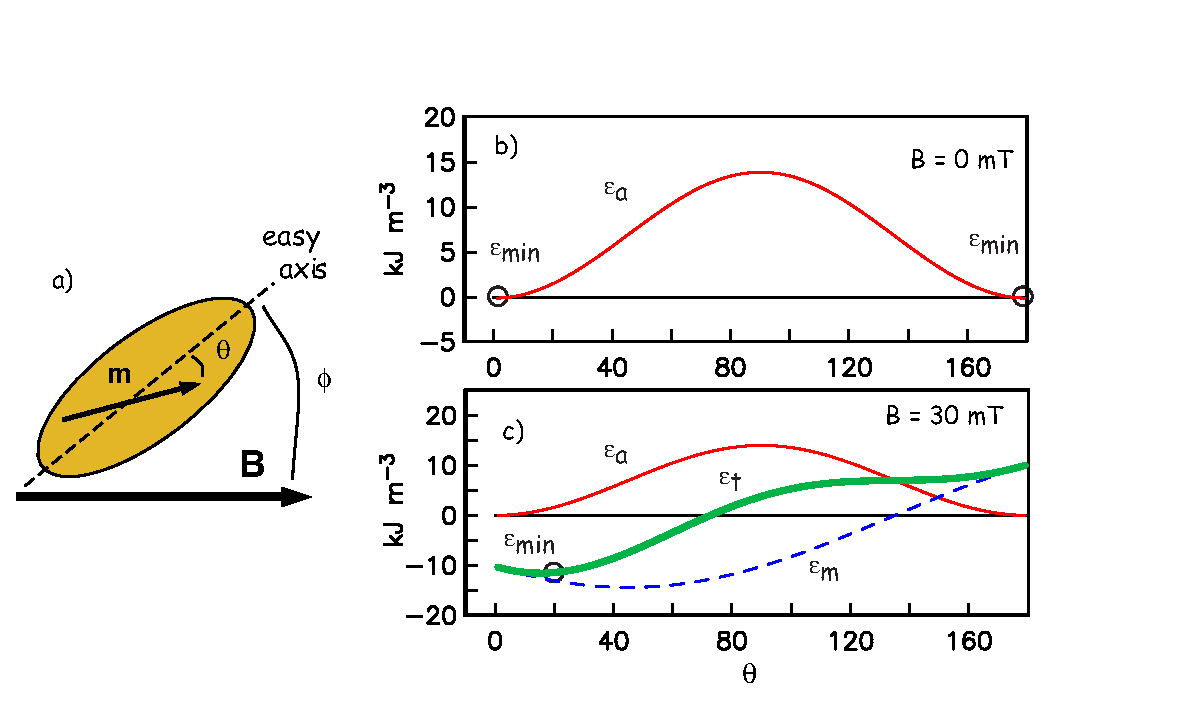
\includegraphics[width=14 cm]{EPSfiles/mB.eps}
\caption{a) Sketch of a magnetic particle with easy axis as shown.  In
response to a magnetic field $\B$, applied at an angle $\phi$ to the easy axis, the
particle moment $\m$ rotates, making an angle
$\theta$ with the easy axis. b) Variation of the anisotropy energy density  $\epsilon_a = K_u\sin^2\theta$ as a function of $\theta$ for the particle with $\phi=45^{\circ}$ as  shown in a). The $\theta$ associated with the minimum energy is indicated by $\epsilon_{min}$.  $B$ = 0 mT.  c) same as in b)  but for $B$ = 30 mT.  Also shown  the interaction energy density  $\epsilon_m=-M_s B\cos (\phi-\theta)$ and the total energy density $\epsilon_t=\epsilon_a+\epsilon_m$.}
\label{fig:mB}
\end{figure}



When an external field is applied at an angle $\phi$ to the easy axis (and an angle $\phi-\theta$ with the magnetic moment; see Figure~\ref{fig:mB}a), the magnetostatic  interaction energy  density $\epsilon_m$  given by the dot product of the magnetization and the applied field (Equation~\ref{eq:Em1}  in Chapter 4) or: 

  $$
\epsilon_m = -\M \cdot \B = -MB \cos(\phi-\theta).
 $$
 
 \noindent
The two energy densities  ($\epsilon_a$ and $\epsilon_m$) are shown as the thin solid and dashed lines  in Figure~\ref{fig:mB}c for an applied field of 30 mT aligned with an angle of 45$^{\circ}$ to the easy axis.   
There is a 
 competition between the anisotropy energy (tending to keep the magnetization parallel to the easy axis) and the interaction energy (tending to line the magnetization up with the external magnetic field).   Assuming that the magnetization is at saturation, we get the total energy density of the particle to be: 

 
\begin{equation}
\epsilon_t = K_u\sin^2\theta - M_s B \cos (\phi-\theta).
\label{eq:Et}
\end{equation}

\noindent  The total energy density $\epsilon_t$ is shown as the heavy solid line in Figure~\ref{fig:mB}c. 



The magnetic moment of a uniaxial single domain grain will find the angle $\theta$ that is associated with the minimum total energy density ($\epsilon_{min}$; see Figure~\ref{fig:mB}b,c).  For low external fields, $\theta$ will be closer to the easy axis  and for higher external fields (e.g., 30 mT; Figure~\ref{fig:mB}c), $\theta$ will be closer to the applied field direction ($\phi$).  



\begin{figure}[h!tb]
%\epsfxsize 14cm
%\centering \epsffile{EPSfiles/flip.eps}
\centering  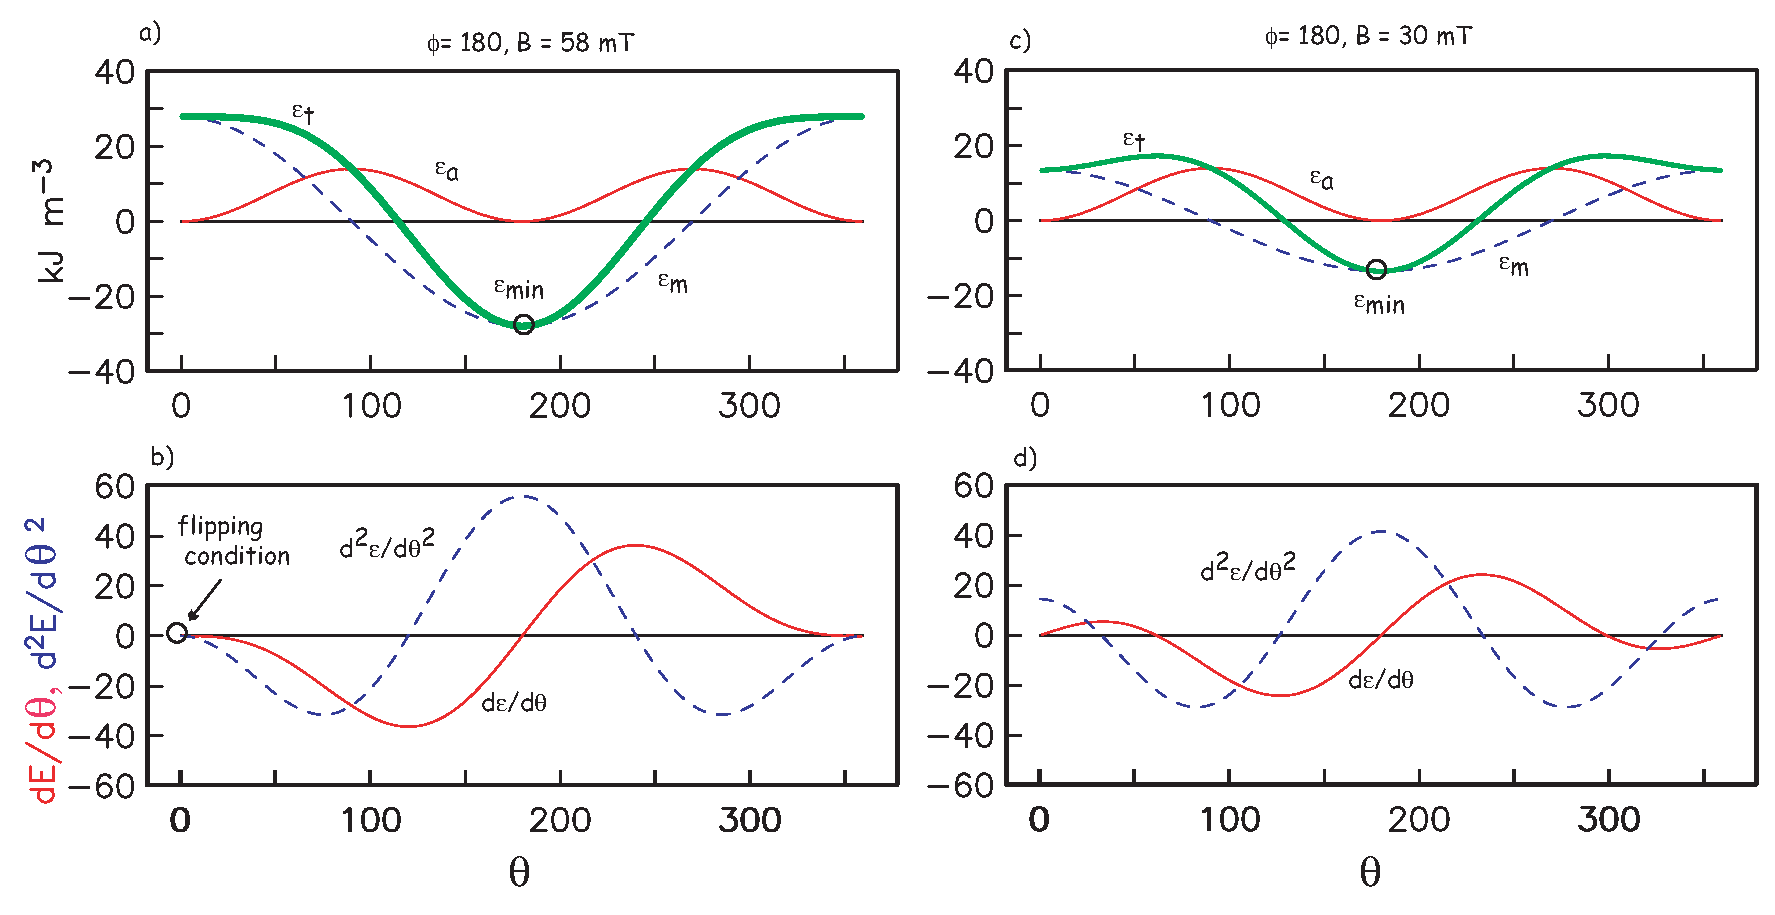
\includegraphics[width=14 cm]{EPSfiles/flip.eps}
\caption{a) Variation of the anisotropy energy density  $\epsilon_a = K_u\sin^2\theta$, the interaction energy density $\epsilon_m=-M_s B\cos \phi$ and the total energy density $\epsilon_t=\epsilon_a+\epsilon_m$ as a function of $\theta$ for the particle shown in Figure 5.1a.  The  field was applied with $\phi$ = 180$^{\circ}$ and was 58 mT in magnitude.  The $\theta$ associated with the minimum energy is indicated by $\epsilon_{min}$ and is 180$^{\circ}$.  b) Variation in first and second derivatives of the energy equation.  The flipping condition of both being zero simulaneously is met.  c) Same as a) but the field was only 30 mT.  d) Same as b but the flipping condition is not met.} 
\label{fig:flip}
\end{figure}


When a  magnetic field  that is large enough to overcome the anisotropy energy is applied in a direction opposite to the magnetization vector, the moment will jump over the energy barrier and stay in the opposite direction when the field is switched off.  The field necessary to accomplish this feat is called the 
\index{flipping!field}
\index{switching field}
{\it flipping field}  ($\mu_oH_f$)  (also sometimes the ``switching field'').    [Note the change to the use of $H$ for internal fields where $M$ cannot be considered  zero.)   \nocite{stoner48}   We introduced this parameter in Chapter 4 (see Equation~\ref{eq:Bk}) as the microscopic coercivity.   
\index{Stoner, C.}
\index{Wohlfarth, W.P.}
Stoner and Wohlfarth (1948)  showed that the flipping field can be found from the condition that $d\epsilon_t/d\theta = 0$ and $d^2\epsilon_t/d\theta^2$ = 0.  We will call this the 
\index{flipping!condition}
``flipping condition''.   The necessary equations can be found by differentiating Equation~\ref{eq:Et}:

\begin{equation}
{d\epsilon \over {d\theta}} = 2 K_u \sin \theta \cos \theta - M_s B \sin (\phi - \theta),
\label{eq:1stderiv}
\end{equation}
\noindent
and again

\begin{equation}
{d^2 \epsilon\over {d\theta^2}} = 2 K_u \cos (2\theta) + M_s B \cos (\phi - \theta ).
\label{eq:2ndderiv}
\end{equation}

\noindent Solving these two equations for $B$ and substituting $\mu_oH$ for $B$,  we get after some trigonometric trickery:

\begin{equation}
\mu_o H_f = { {2K_u \over {M_s} } 
{  {(1-t^2 + t^4)^{1\over 2} } \over {1 + t^2} } }=   {2K_u \over {M_s} }
{ 1 \over { (\cos ^{2\over 3}  \phi + \sin ^{2\over 3} \phi)^{3\over 2} }},
\label{eq:Bf}
\end{equation}

\noindent where $t= \tan^{1\over 3} \phi$.  In this equation, $\phi$ is the angle between the applied field and the easy axis direction opposite to $m$.    

Now we can derive  the so-called 
\index{coercivity!microscopic}
 ``microscopic coercivity'' ($H_k$)  introduced in  Section~\ref{sect:coercivity} in Chapter 4.  Microscopic coercivity is the maximum flipping field for a particle.    When  magnetic anisotropy  of a  particle is dominated by uniaxial anisotropy constant $K_u$ and $\phi$ is zero (antiparallel to the easy direction nearest the moment),   $\mu_o H_k = 2{ {K_u}\over {M_s} }$.     
Using the values appropriate for magnetite ($K_u$ = 1.4 x 10$^4$ Jm$^{-3}$ and $M_s$ = 480 mAm$^{-1}$ we get $\mu_o H_k$ = 58 mT.  To see why this would indeed result in a flipped moment, we plot the behavior of Equations~\ref{eq:Et} - \ref{eq:2ndderiv} in Figure~\ref{fig:flip}.  The minimum in total energy $\epsilon_t$ occurs at an angle of $\theta$ = 180$^{\circ}$ (Figure~\ref{fig:flip}a) and the first and second derivatives satisfy the flipping condition by having a common zero crossing ($\theta=0$ in Figure~\ref{fig:flip}b).   There is no other applied field value for which this is true (see, e.g., the case of  a 30 mT field in Figure~\ref{fig:flip}c,d). 

\begin{figure}[h!tb]
%\epsfxsize 7cm
%\centering \epsffile{EPSfiles/bf.eps}
\centering  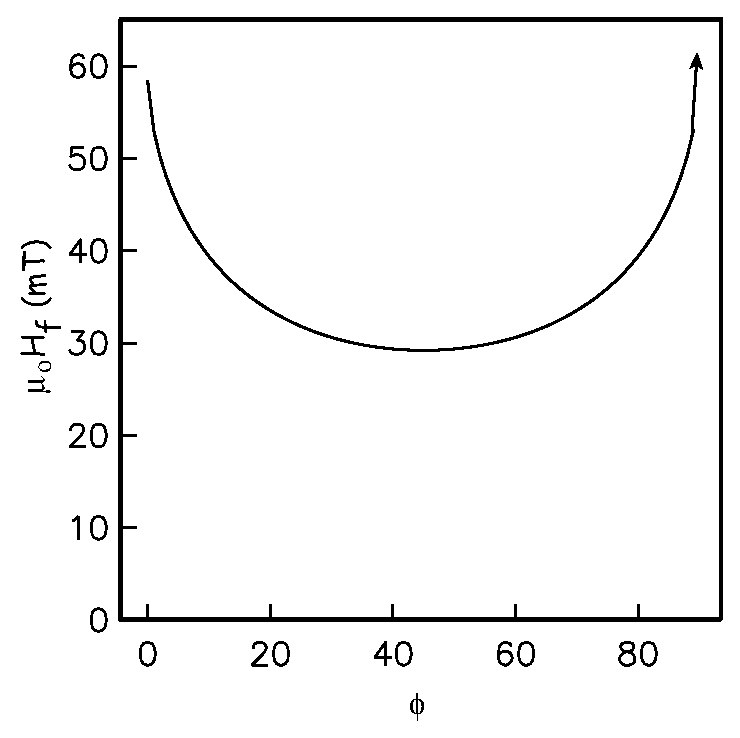
\includegraphics[width=7 cm]{EPSfiles/bf.eps}
\caption{The flipping field $\mu_oH_f$ required to irreversibly switch the magnetization vector from one easy direction to the other in a single domain particle dominated by uniaxial anisotropy. Note that $\phi$ is the angle with the easy axis, but must be the opposite direction from $\textbf{m}$.   }
\label{fig:bf}
\end{figure}


The flipping condition depends not only on the applied field magnitude but also on  the direction that it makes with the easy axis   (see $\mu_oH_f$ versus $\phi$ in Figure~\ref{fig:bf}).  When $\phi$ is parallel to the easy axis (zero) (and anti-parallel to $\textbf{m}$, $\mu_oH_f$ is  58 mT as we found before.  $\mu_oH_f$ drops steadily as the angle between the field and the easy axis increases until an angle of 45$^{\circ}$ when $\mu_oH_f$ starts to increase again.   According to Equation~\ref{eq:Bf}, $\mu_oH_f$ is undefined when $\phi$ = 90$^{\circ}$, so when the field is applied at right angles to the easy axis, there is no field sufficient to flip the moment. 


\section{Hysteresis loops}

In this section we will develop the theory for predicting  the response of substances to the application of external fields, in experiments that generate hysteresis loops.  We will define a number of parameters which are useful in rock and paleomagnetism.   For computational details in estimating these parameters from hysteresis data, see Appendix~\ref{app:hyst}.

Let us begin by considering  what happens to single particles when subjected to applied fields in the cycle known as the
\index{hysteresis!loops}
{\it hysteresis loop}.   From the last section,  we know that when a single domain, uniaxial particle is subjected to an increasing magnetic field the magnetization is gradually drawn into the direction of the applied field.  If the flipping condition is not  met, then the magnetization will return to the original direction when the magnetic field is removed.  If the flipping condition is met, then the magnetization undergoes an irreversible change and will be  in the opposite direction when the magnetic field is removed.       




\subsection{Uniaxial anisotropy}
\label{sect:uniaxial}

Imagine a single domain particle with 
\index{anisotropy!uniaxial}
uniaxial anisotropy.   Because the particle is single domain, the magnetization is at saturation and, in  the absence of an applied field is constrained to lie along the easy axis.  Now suppose we apply a magnetic field in the opposite direction (see track \# 1 in  Figure~\ref{fig:outerloop}a).  When $B$ reaches $\mu_oH_f$ in magnitude, the magnetization flips to the opposite direction (track \#2 in  Figure~\ref{fig:outerloop}) and will not change further regardless of how high the field goes.  The field then is decreased to zero and then increased along track \#3 in  Figure~\ref{fig:outerloop} until $\mu_oH_f$ is reached again.  The magnetization then flips back to the original direction (track \#4 in  Figure~\ref{fig:outerloop}a).    




Applying fields at arbitrary angles to the easy axis results in loops of various shapes (see Figure~\ref{fig:outerloop}b).   As $\phi$ approaches 90$^{\circ}$, the loops become thinner.  Remember that the flipping fields for $\phi$ = 22$^{\circ}$ and $\phi = 70^{\circ}$ are similar (see Figure~\ref{fig:bf}) and are lower than that when $\phi=0^{\circ}$, but the flipping field for $\phi = 90^{\circ}$ is infinite, so that ``loop'' is closed and completely reversible.  


\begin{figure}[h!tb]
%\epsfxsize 14cm
%\centering \epsffile{EPSfiles/outerloop.eps}
\centering  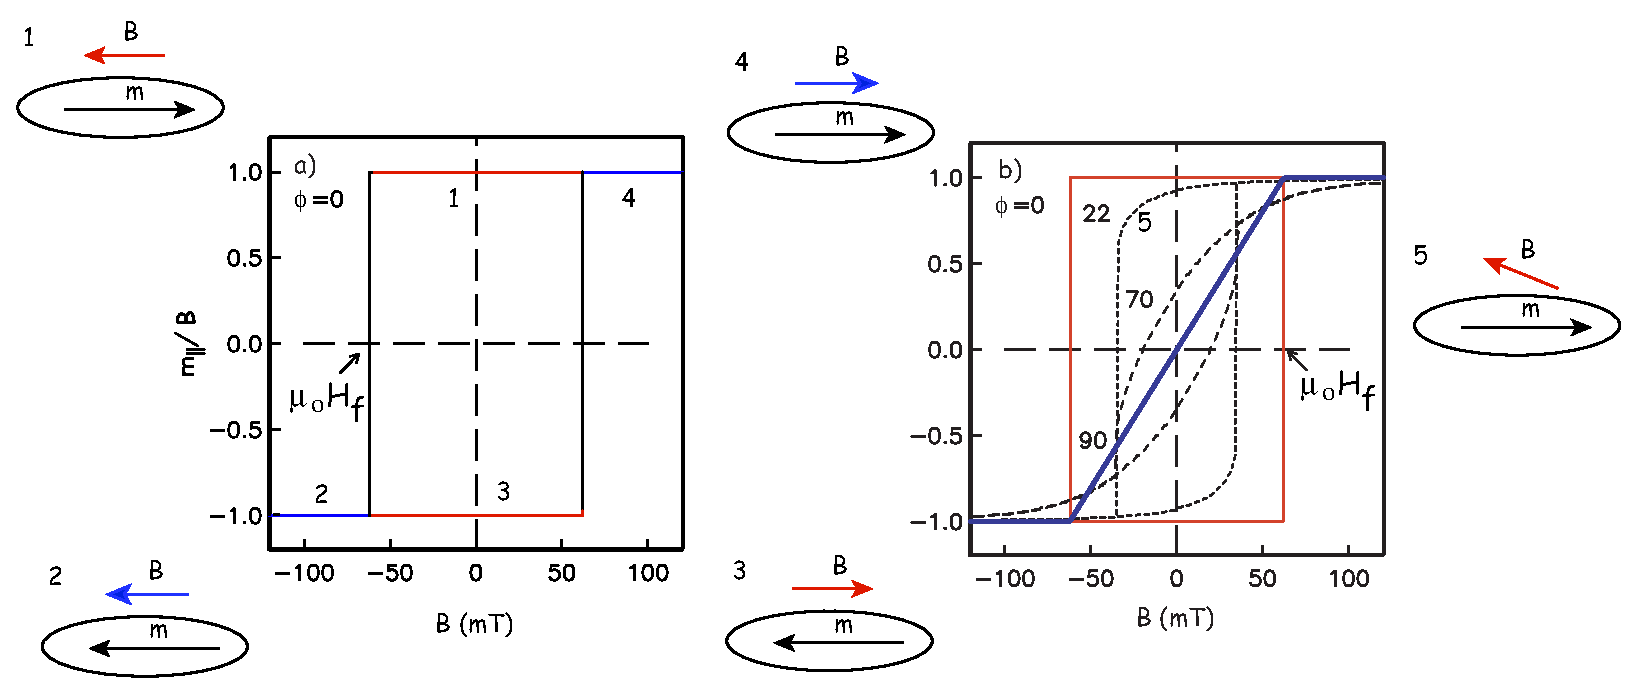
\includegraphics[width=14 cm]{EPSfiles/outerloop.eps}
\caption{ Moment measured for the particle ($\phi=0^{\circ}$) with applied field starting at 0 mT and increasing in the opposite directions along track \#1.  When the flipping field $\mu_oH_f$ is reached, the moment switches to the other direction along track \#2.  The field then switches sign and decreases along track \#3 to zero, then increases again to the flipping field.  The moment flips and the the field increases along track \#4. b) The component of magnetization  parallel to +B$_{max}$ versus $B$ for field applied with various angles $\phi$.  }
\label{fig:outerloop}
\end{figure}




Before we go on, it is useful to consider for a moment how 
\index{hysteresis!measurement of}
hysteresis measurements are made in practice.  
Measurements of magnetic moment $m$ as a function of applied field $B$ are made on a variety of instruments, such as a 
\index{magnetometer!vibrating sample}
\index{magnetometer!alternating gradient force}
vibrating sample magnetometer (VSM) or alternating gradient force magnetometer (AGFM).  In the latter, a specimen is placed on a thin stalk between pole pieces of a large magnet.  There is a probe mounted  behind the specimen that measures the applied magnetic field.  There are small coils on the pole pieces that modulate the gradient of the applied magnetic field (hence alternating gradient force).   The specimen vibrates in response to changing magnetic fields and the amplitude of the vibration is proportional to the moment in the axis of the applied field direction.   The vibration of the specimen stalk is measured and calibrated in terms of magnetic moment.  The magnetometer is only sensitive to the
induced 
component of $\m$ parallel to the applied field $\B_o$, which is  $m_{||}= m \cos \phi$ (because the off axis terms are squared and very small, hence can be neglected.) 
In the hysteresis experiment, therefore,  the moment parallel to the field $m_{||}$ is measured as a function of applied field $B$.  


\begin{figure}[h!tb]
%\epsfxsize 14cm
%\centering \epsffile{EPSfiles/sdloops.eps}
\centering  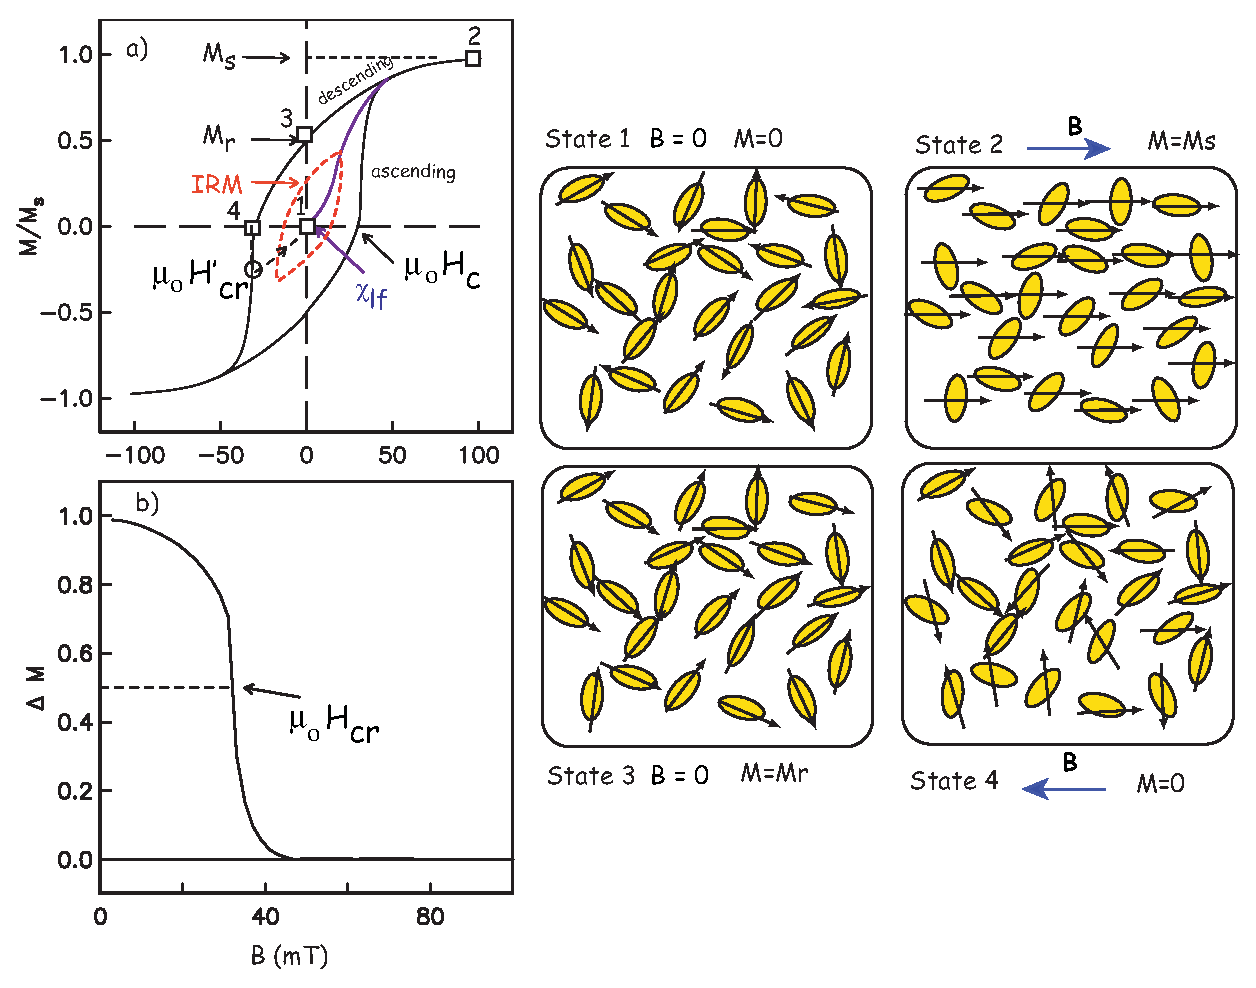
\includegraphics[width=14 cm]{EPSfiles/sdloops.eps}
\caption{a)  Net response of a random assemblage of  uniaxial single domain particles.  Snap shots of magnetization states (squares labelled 1 to 4)  for representative particles  are shown in the balloons labelled State 1- 4.   The initial demagnetized state is ``State 1''.  The initial slope as the field is increased from zero is the low-field susceptibility $\chi_{lf}$.      If the field returns to zero after some flipping fields have been exceeded, there is a net 
\index{magnetization!remanent!isothermal}
isothermal remanence (IRM).   When all the moments are parallel to the applied field (State 2), the magnetization is at saturation $M_s$. When the field is returned to zero, the magnetization is a saturation remanence ($M_r$; State 3).    When the field is applied in the opposite direction and has remagnetized half the moments (State 4), the field is the  bulk coercive field $\mu_oH_c$.   When a field is reached that when reduced to zero leaves zero net remanence, that field is  the coercivity of remanence (here labelled $\mu_oH_{cr}'$).    b)  Curve obtained by subtracting the ascending curve in a)  from the descending curve.  The field at which half the moments have flipped, leaving a magnetization of one half of saturation is another measure of the coercivity of remanence, here labelled $\mu_oH_{cr}$.}
\label{fig:sdloops}
\end{figure}


In rocks with an assemblage of randomly oriented particles with uniaxial anisotropy, we would measure the sum of all the millions of tiny individual loops.  A specimen from such a rock would yield a loop similar to that shown in Figure~\ref{fig:sdloops}a.  If the field is first applied to a demagnetized specimen, the initial slope is the (low field) 
\index{magnetic!susceptibility!low field}
magnetic susceptibility ($\chi_{lf}$) first introduced in  Chapter 1.   From the treatment in Section~\ref{sect:flipping} it is possible to derive the equation $\chi_{lf} = \mu_o M_s^2/3K_u$ for this initial (ferromagnetic) susceptibility (for more, see
\nocite{oreilly84}
\index{O'Reilly,  O.}
O'Reilly 1984). 



 If the field is increased beyond the flipping field of some of the magnetic grains and returned to zero, the net remanence is called an 
 \index{magnetization!remanent!isothermal}
{\it isothermal remanent magnetization} (IRM).  If the field is increased to $+B_{max}$, all the magnetizations are drawn into the field direction and the net magnetization is equal to the sum of all the individual magnetizations and is the {\it saturation magnetization} $M_s$.    When the field is reduced to zero, the moments relax back to their individual easy axes, many of which are at a high angle to the direction of the saturating field and cancel each other out.   A loop that does not achieve a saturating field (red in Figure~\ref{fig:sdloops}a is called a {\it minor hysteresis loop}, while one that does is called the {\it outer loop}. 
 
 
\begin{figure}[htb]
%\epsfxsize 7.75cm
%\centering \epsffile{EPSfiles/Bcr.eps}
\centering  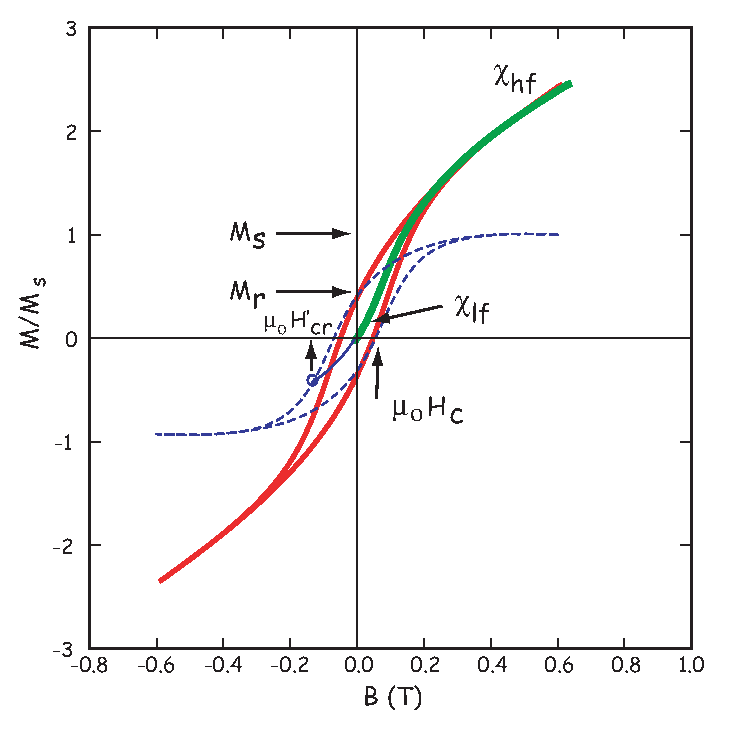
\includegraphics[width=7.75 cm]{EPSfiles/Bcr.eps}
\caption{Heavy green line: initial behavior of demagnetized specimen as applied field ramps up from zero field to a saturating field.  The initial slope is the initial or low-field susceptibility $\chi_{lf}$.  After saturation is achieved the slope is the high-field susceptibility $\chi_{hf}$ which is the non-ferromagnetic contribution, in this case the paramagnetic susceptibility (because $\chi_{hf}$ is positive.) The dashed blue line is the hysteresis loop after the paramagnetic slope has been subtracted.  Saturation magnetization $M_s$ is the maximum value of magnetization after slope correction.  Saturation remanence $M_r$ is the value of the magnetization remaining in zero applied field.  Coercivity ($\mu_o H_c$) and coercivity of remanence $\mu_oH_{cr}'$ are as in Figure 5.5a. }
 \label{fig:Bcr}
\end{figure}

%\clearpage

The net remanence after saturation is termed the 
 \index{magnetization!remanent!saturation}
{\it saturation remanent magnetization} $M_r$ (and sometimes the saturation isothermal remanence sIRM).  For a random assemblage of single domain uniaxial particles, $M_r/M_s$ = 0.5.   The field necessary to reduce the net moment to zero is defined as the 
\index{coercive field}
{\it coercive field} ($\mu_oH_c$) (or coercivity).  




The 
\index{coercivity!of remanence}
coercivity of remanence $\mu_o H_{cr}$ is defined as the magnetic field required to irreversibly flip half the magnetic moments (so the net remanence after application of a field equal to $-\mu_oH_{cr}$ to a saturation remanence is 0).  The coercivity of remanence is always greater than or equal to the coercivity and the ratio $H_{cr}/H_c$ for our random assemblage of uniaxial SD particles is 1.09
 \nocite{wohlfarth58}    
 \index{Wohlfarth, W.P.}
 (Wohlfarth, 1958).   Here we introduce two ways of estimating coercivity of remanence, illustrated in Figure~\ref{fig:sdloops}.  
 \index{coercivity!of remanence!estimation!ascending loop intercept method}
  If, after taking the field up to some saturating field $+B_{max}$, one first turned the field off (the descending curve), then increased the field in the opposite direction to the point labeled $\mu_oH'_{cr}$, 
and one were to then switch the field off again, the magnetization would follow the dashed curve up to the origin.   For single domain grains, the dashed curve would be  parallel to the lower curve (the ascending curve).  So, if one only measured the outer loop, one could estimate the coercivity of remanence by simply tracing the curve parallel to the lower curve (dashed line) from the origin to the point of intersection with the upper curve (circled in Figure~\ref{fig:sdloops}a).    This estimate is only valid for single domain grains, hence the prime in $\mu_oH_{cr}'$.   



 

 An alternative means of estimating coercivity of remanence  is to use  a so-called 
 \index{coercivity!of remanence!estimation!$\Delta M$ method}
 $\Delta M$ curve 
 \nocite{jackson90} 
 \index{Jackson, M.J.}
 (Jackson et al., 1990) which is obtained by subtracting the  ascending loop  from the descending loop (see  Figure~\ref{fig:sdloops}b).  When all the moments are flipped into the new field, the ascending and descending loops join together and $\Delta M$ is 0.  $\Delta M$ is at 50\% of its initial value at the field at which  half the  moments are flipped (the definition of coercivity of remanence); this field is here termed $\mu_oH_{cr}$.   
 



\subsection{Magnetic susceptibility}
\label{sect:chi}

Figure~\ref{fig:sdloops}a is the loop created in the  idealized case in which only uniaxial ferromagnetic particles participated in the hysteresis measurements; in fact the curve is entirely theoretical.  In ``real'' specimens there can be  paramagnetic, diamagnetic AND ferromagnetic particles and the loop may well look like that shown in Figure~\ref{fig:Bcr}.   The initial slope of a hysteresis experiment starting from a demagnetized state in which the field is ramped from zero up to higher values is the low field magnetic susceptibility or $\chi_{lf}$ (see Figure~\ref{fig:Bcr}).   If the field is then turned off, the magnetization will return again to zero.  But as the field increases passed the lowest flipping field, the remanence will no longer be zero but some isothermal remanence.    Once all particle moments have flipped and saturation magnetization has been achieved, the slope relating magnetization and applied field  reflects only the non-ferromagnetic (paramagnetic and/or diamagnetic)  susceptibility, here called
\index{magnetic!susceptibility!high field}
 {\it high field susceptibility}, $\chi_{hf}$.   In order to estimate the 
 \index{magnetization!saturation}
 saturation magnetization and the 
 \index{magnetization!remanent!saturation}
 saturation remanence, we must first subtract the high field slope.  So doing gives us the blue dashed line in Figure~\ref{fig:Bcr} from which we may read the various hysteresis parameters illustrated in Figure~\ref{fig:sdloops}b.  



\subsection{Cubic anisotropy}

In the case of  equant grains of magnetite for which magnetocrystalline anisotropy dominates, there are four easy axes, instead of two as in the uniaxial case (see Chapter 4).    The maximum angle $\phi$ between an easy axis and an applied field direction is 55$^{\circ}$.  Hence there is no individual loop that goes through the origin (see Figure~\ref{fig:cubic}).    A random assemblage of particles with 
\index{anisotropy!cubic}
cubic anisotropy will therefore have a much higher saturation remanence.  In fact, the theoretical ratio of $M_r/M_s$  for such an assemblage is 0.87, as opposed to 0.5 for the uniaxial case 
\nocite{joffe74}
\index{Joffe, I.}
\index{Heuberger, R.}
(Joffe and Heuberger, 1974).      
\begin{figure}[h!tb]
%\epsfxsize 6cm
%\centering \epsffile{EPSfiles/cubicloops.eps}
\centering  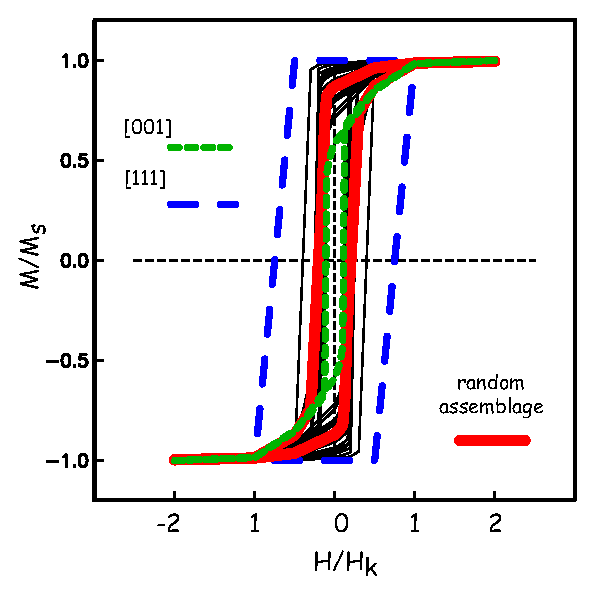
\includegraphics[width=6 cm]{EPSfiles/cubicloops.eps}
\caption{Heavy lines: theoretical behavior of cubic grains of magnetite.  Dashed lines are the responses along particular directions.  Light grey lines: hysteresis response for single particles with various orientations with respect to the applied field. [Figure from Tauxe et al., 2002.]}
\label{fig:cubic}
\end{figure}  
\nocite{tauxe02}


\begin{figure}[htb]
%\epsfxsize 12cm
%\centering \epsffile{EPSfiles/loops.eps}
\centering  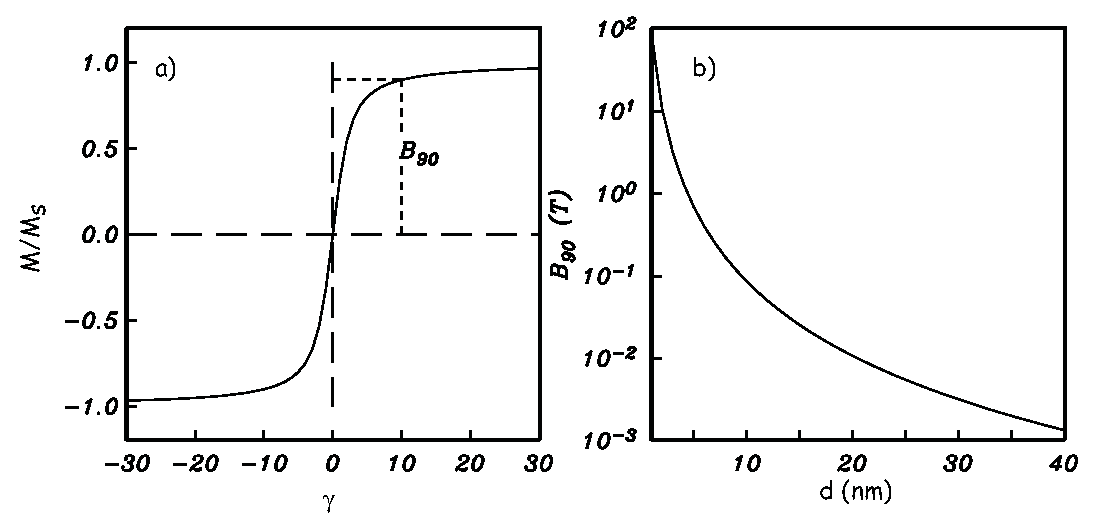
\includegraphics[width=12 cm]{EPSfiles/loops.eps}
\caption{a) The contribution of SP particles with saturation magnetization $M_s$ and cubic edge length $d$.  $\gamma = BM_s d^3/kT$.  There is no hysteresis.  b) The field at which the magnetization reaches 90\% of the maximum $B_{90}$ is when $ M_s d^3/kT\simeq 10$. [Figure from Tauxe et al.,  1996.] }
\label{fig:loops}
\end{figure}
\nocite{tauxe96}

\subsection {Superparamagnetic particles}
\label{sect:SP}

In 
\index{superparamagnetism}
superparamagnetic (SP) particles, the total magnetic energy $E_t=\epsilon_tv$ (where $v$ is volume) is balanced by thermal energy $kT$.  This behavior can be modeled using statistical mechanics  in a manner similar to that derived for paramagnetic grains in Section~\ref{sect:para} in Chapter 3 and summarized in Appendix~\ref{app:superparamagnetism}.  In fact, 


\begin{equation}
{M\over {M_s}} =
{ N(\hbox{coth }\gamma -
{
1\over{\gamma}
}), 
}
\label{eq:Lang1} 
\end{equation}
\noindent where $\gamma = { {M_sBv}\over {kT}} $ and $N$ is the number of particles of volume $v$, 
 is a reasonable approximation. 
The end result, Equation~\ref{eq:Lang1}, is the familiar 
\index{Langevin!function}
Langevin function from our discussion of  paramagnetic behavior (see Chapter  3); hence
the   term ``superparamagnetic'' for such particles.

 



The
contribution of SP particles for which the Langevin function is valid with given $M_s$ and $d$ is shown in Figure~\ref{fig:loops}a.
The field at which the population reaches 90\%
saturation $B_{90}$ occurs at $\gamma \sim 10$.  
Assuming particles of magnetite ($M_s$ = 480 mAm$^{-1}$) and room temperature 
($T=300$\deg K), $B_{90}$ can
be evaluated as a function of $d$ (see Figure~\ref{fig:loops}b). 
Because of its inverse cubic dependence on $d$, $B_{90}$ rises sharply with decreasing $d$ and is
hundreds of tesla for particles a few nanometers in size, approaching paramagnetic
values.    $B_{90}$ is a quick guide to the  SP slope (the SP susceptibility $\chi_{sp}$) contributing to the hysteresis response and was  used by Tauxe et al. (1996) \nocite{tauxe96} as a means of explaining distorted loops sometimes observed for populations of SD/SP mixtures.   $B_{90}$ (and $\chi{sp}$) is  very sensitive to particle size with very steep slopes for the particles at the SP/SD threshold.   The exact threshold size 
is still rather controversial, but Tauxe et al. (1996) argue that it is $\sim $ 20 nm. 
\eject

\begin{figure}[htb]
%\epsfxsize 14cm
%\centering \epsffile{EPSfiles/mdloop.eps}
\centering  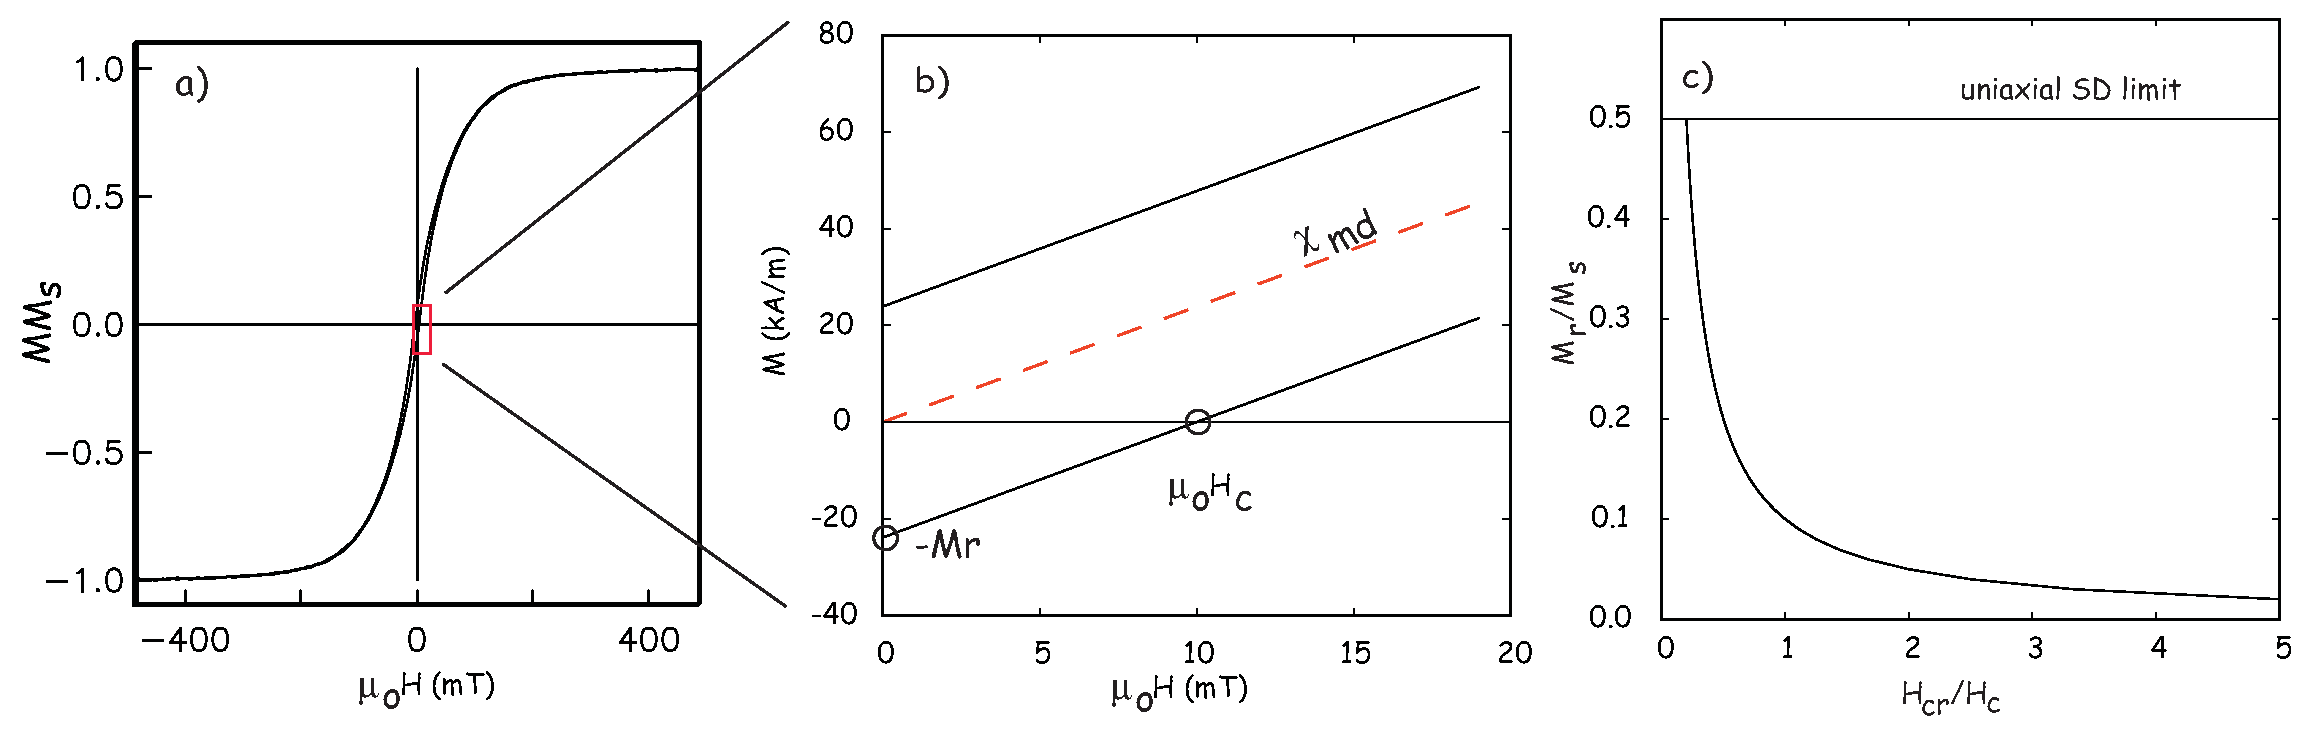
\includegraphics[width=14 cm]{EPSfiles/mdloop.eps}
\caption{a) Typical hysteresis loop from a multi-domain assemblage.   b) Theoretical behavior for the region in the inset to a).  c) Theoretical relationship between $M_r/M_s$ and $H_{cr}/H_c$ for constant $\chi_iH_c/M_s = 0.1$.   Heavy red line is the theoretical linear mixing curve of SD/MD end-members.  (see text) }
\label{fig:md}
\end{figure}


For low magnetic fields, the Langevin function can be approximated as $\sim 1\over 3 \gamma$.  So we have:
$$
{M\over {M_s}} = {1\over 3}  { {M_sBv}\over {kT}}.
$$
\noindent   If we substitute $\mu_o H$ for $B$ and rearrange this equation, we can get the superparamagnetic susceptibility $\chi_{sp}$ as:
\beq
{M\over H} =   { {\mu_o M_sv}\over {3kT}}.
\label{eq:chiSP}
\eeq

\noindent We can rearrange  Equation~\ref{eq:tau} in Chapter 4 to solve for the volume at which a uniaxial grain passes through the superparamagnetic threshold we find:  

$$
{v_b } ={{ \ln (C\tau)}\over{K_u}}.
$$
\noindent Finally, we  can substitute this volume into Equation~\ref{eq:chiSP} as the maximum volume of an SP grain, giving us:

\beq
\chi_{sp} = { {\mu_o M_s^2 \ln (C\tau)}\over {3K_u} }.
\label{eq:chiSP1}
\eeq

\noindent Comparing this expression with that derived for ferromagnetic susceptibility in Section~\ref{sect:uniaxial}, we find that $\chi_{sp}$ is a factor of $\ln(C\tau)\simeq 27$ larger than the equivalent single domain particle.  



 \begin{figure}[htb]
%\epsfxsize 12cm
%\centering \epsffile{EPSfiles/void.eps}
\centering  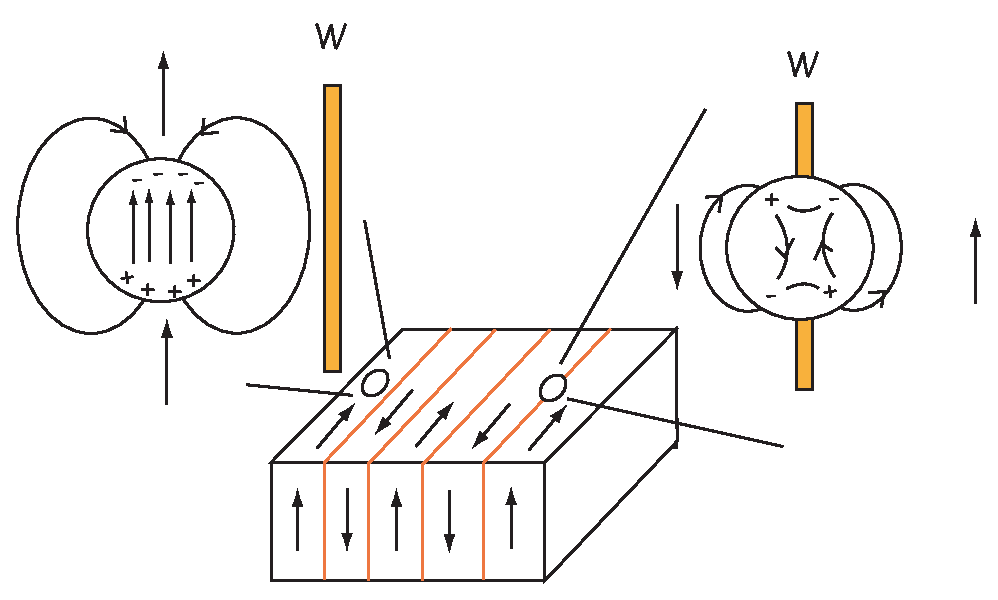
\includegraphics[width=12 cm]{EPSfiles/void.eps}
\caption{ Interaction of a domain wall and a void.  When the void is within a domain, free poles create a magnetic field which creates a self energy (Chapter 4).  When a domain wall intersects the void, the self-energy is reduced.  There are no exchange or magnetocrystalline anisotropy energy terms within the void, so the wall energy is reduced.}
\label{fig:void}
\end{figure}




\subsection{Particles with domain walls}
\label{sect:day}


Moving domain walls around is much easier than flipping the magnetization of an entire particle coherently.   The reason for this is the same as the reason that it is easier to move a rug by lifting up a small wrinkle and pushing that through the rug, than to drag the whole rug by the same amount.  Because of the greater ease of changing magnetic moments in multidomain (MD) grains, they have lower coercive fields and saturation remanence is also much lower than for uniformly magnetized particles (see typical MD hysteresis loop in Figure~\ref{fig:md}a.)

The key to understanding multi-domain hysteresis is the reduction in multi-domain magnetic susceptibility  $\chi_{md}$ from ``true'' magnetic susceptibility ($\chi_i$) because of self-demagnetization.  The true susceptibility would be that obtained by measuring the magnetic response of a particle to the internal field $\H_i$ (applied field minus the demagnetizing field $-N\M$ -- see Section~ \ref{sect:shape}; see 
\index{Dunlop, D.J.}
Dunlop 2002a).  \nocite{dunlop02a}
  Recalling that the demagnetizing factor is $N$, the so-called {\it screening factor} $f_s$ is $(1 + N\chi_i)^{-1}$ and $\chi_{md} = f_s \chi_i $.
If we assume that $\chi_{md}$ is linear for fields less than the coercivity, then by definition $\chi_{md} = {{ M_r}\over{H_c} }$ (see Figure~\ref{fig:md}b).  From this, we get:

$$
{{M_r}\over{M_s}} = \chi_{md} { H_c\over{M_s}} = f_s \chi_i { H_c\over{M_s}}.
$$
\noindent In the case of multi-domain susceptibility,  $\chi_i$ is much larger than $\chi_{md}$ and $M_r = { {H_c}\over{N}}$.    

By a similar argument,
\index{coercivity!of remanence}
coercivity of remanence ($H_{cr}$) is suppressed by the  screening factor which gives coercivity so:

$$
H_c =  f_s H_{cr}, 
$$
\noindent    from which we get the ratio:

$$
{H_{cr}\over{H_c}} = f_s. 
$$
\noindent  

\noindent Putting all this together leads us to the remarkable relationship noted by 
\index{Day, R.}
Day et al. (1977; see also 
\index{Dunlop, D.J.}
Dunlop 2002a): \nocite{day77,dunlop02a} 

\begin{equation}
{ M_r\over{M_s}} \cdot { H_{cr}\over{H_c}} = \chi_i { H_c\over {M_s}}.
\label{eq:day}
\end{equation} 

When  $\chi_i { H_c\over {M_s}}$ is constant, Equation~\ref{eq:day} is a hyperbola.   
For a single mineralogy, we can expect $M_s$ to be constant, but $H_c$ depends on grain size and the state of stress which are unlikely to be constant for any natural population of magnetic grains.   
\index{Dunlop, D.J.}
Dunlop (2002a) \nocite{dunlop02a} argues that if the main control on susceptibility and coercivity is domain wall motion through a terrain of variable wall energies, then $\chi_i$ and $H_c$ would be inversely related and gives a tentative theoretical value for $\chi_iH_c$  in magnetite of  about 45 kAm$^{-1}$.   This, combined with the value of $M_s$ for magnetite of 480  kAm$^{-1}$  gives a value for $\chi_i { H_c\over {M_s}} \sim 0.1$.  
When anchored by the theoretical maximum for uniaxial single domain ratio of $M_r/M_s = 0.5$, we get the curve shown in Figure~\ref{fig:md}c.   The major control on coercivity is grain size, so the trend from the SD limit down toward low $M_r/M_s$ ratios is increasing grain size.  

   
  

There are several possible causes of variability in wall energy within a magnetic grain, for example, voids, lattice dislocations, stress, etc.  The effect of voids is perhaps the easiest to visualize, so we will consider voids as an example of why wall energy varies as a function of position within the grain.   We show a particle with lamellar domain structure and several voids in Figure~\ref{fig:void}.  When the void occurs within a uniformly magnetized domain (left of figure), the void sets up a demagnetizing field as a result of the free poles on the surface of the void.  There is therefore, a self-energy associated with the void.   When the void is traversed by a wall, the free pole area is reduced, reducing the demagnetizing field and the associated self-energy.  Therefore, the energy of the void is reduced by having a wall bisect it.  Furthermore, the energy of the wall is also reduced, because the area of the wall in which magnetization vectors are tormented by exchange and magnetocrystalline energies is reduced.  The wall gets a ``free'' spot if it bisects a void.  The wall energy $E_w$ therefore is lower as a result of the void.  




\begin{figure}[htb]
%\epsfxsize 14cm
%\centering \epsffile{EPSfiles/wallenergy.eps}
\centering  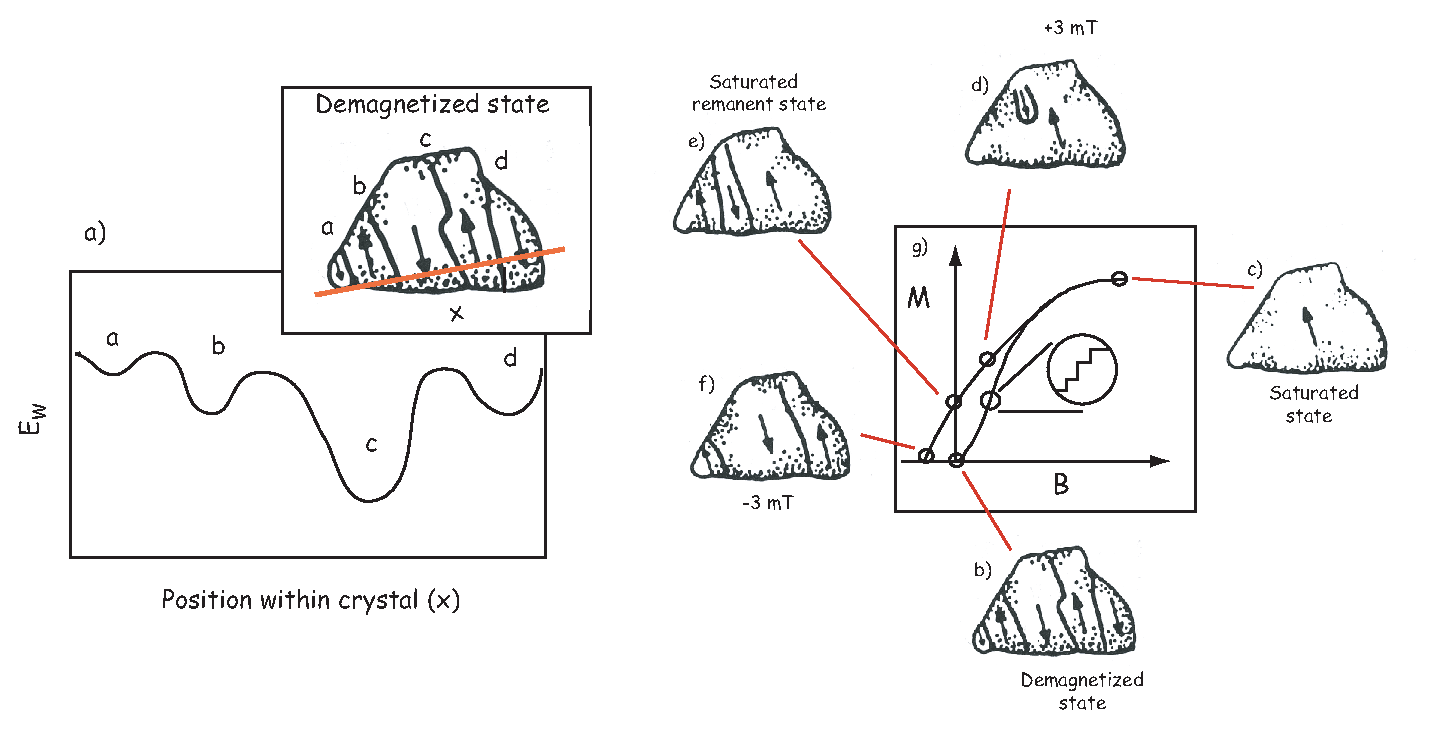
\includegraphics[width=14 cm]{EPSfiles/wallenergy.eps}
\caption{a) Schematic view of wall energy across a transect of a multi-domain grain.  Inset: Placement of domain walls in the demagnetized state.  [Domain observations from Halgedahl and Fuller,  1983.] b-g) Schematic view of the magnetization process in MD grain shown in previous figure.  b) Demagnetized state, c) in the  presence of a saturating field, d) field lowered to +3 mT, e) remanent state, f) backfield of -3 mT, g) resulting loop.  Inset shows detail of domain walls moving by small increments called Barkhausen jumps.  [Domain wall observations from Halgedahl and Fuller, 1983; schematic loop after O'Reilly, 1984.]}
\label{fig:wallenergy}
\end{figure}
\nocite{oreilly84}\nocite{halgedahl83}



In  Figure~\ref{fig:wallenergy}, we show a sketch of a hypothetical transect of  $E_w$ across a particle.  There are four LEMs labelled a-d.   Domain walls will distribute themselves through out the grain in order to minimize the net magnetization of the grain and also to try to take advantage of LEMs in wall energy.   

Domain walls move in response to external magnetic fields (see Figure~\ref{fig:wallenergy}b-g).   Starting in the demagnetized state  (Figure~\ref{fig:wallenergy}b), we apply a magnetic field that increases to saturation (Figure~\ref{fig:wallenergy}c).    As the field increases, the domain walls move in sudden jerks as each successive local wall energy high is overcome.  This process, known as {\it Barkhausen jumps},  leads to the stair-step like increases in magnetization (shown in the inset of  Figure~\ref{fig:wallenergy}g).  At saturation, all the walls have been flushed out of the crystal and it is uniformly magnetized.  When the field decreases again, to say +3 mT (Figure~\ref{fig:wallenergy}d), domain walls begin to nucleate, but because the energy of nucleation is larger than the energy of denucleation, the grain is not as effective in cancelling out the net magnetization, hence there is a net saturation remanence (Figure~\ref{fig:wallenergy}e).  The  walls migrate around as a magnetic field is applied in the opposite direction (Figure~\ref{fig:wallenergy}f) until there is no net magnetization.  The difference in nucleation and denucleation energies was called on by \nocite{halgedahl83}
\index{Halgedahl, S.}
\index{Fuller, M.}
Halgedahl and Fuller (1983) to explain the high stability observed in some large magnetic grains. 

\section{Hysteresis of mixtures of SP, SD and MD grains}
\label{sect:mixtures}

\index{Day, R.}
Day et al. (1977) \nocite{day77}  popularized the use of diagrams like that shown in Figure~\ref{fig:md}c which are known as
\index{diagrams!Day}
{\it Day diagrams}.   They placed quasi-theoretical bounds on the plot whereby points with $M_r/M_s$ ratios above 0.5 were labelled  single domain  (SD), and points falling in the box bounded by $0.5>M_r/M_s>0.05$ and $1.5<H_{cr}/H_c < 5$ were labelled
 \index{pseudo-single domain}
{\it pseudo-single domain}  (PSD).  Points with $M_r/Ms$ below 0.05 were labelled multi-domain (MD).    This paper has been cited over 800 times in the literature and the Day plot still serves as the principle way that rock and paleomagnetists determined domain state and grain size.  

The problem with the Day diagram is that virtually all paleomagnetically useful specimens yield hysteresis ratios that fall within the PSD box.  In the early 90s, paleomagnetists began to realize that many  things besides the trend from SD to MD behavior that  control where points fall on the Day diagram.   
\index{Pick, T.}
\index{Tauxe, L.}
Pick and Tauxe (1994) \nocite{pick94} pointed out that mixtures of SP and SD grains would have reduced $M_r/M_s$ ratios and enhanced $H_{cr}/H_c$ ratios. 
\index{Tauxe, L.}
 Tauxe et al. (1996) \nocite{tauxe96} modelled distributions of SP/SD particles and showed that the SP-SD trends always fall above those observed from MD particles (modelled in Figure~\ref{fig:md}c).  

\index{Dunlop, D.J.}
Dunlop (2002a)  \nocite{dunlop02a} argued  that because $M_r$ for SP grains is zero, the  suppression of the ratio $M_r/M_s$ is directly proportional to the volume fraction of the SP particles.  Moreover, 
\index{coercivity!of remanence}
coercivity of remanence remains unchanged, as it is entirely due to the non-SP fraction.    Deriving the relationship of coercivity, however, is not so simple.   It depends on the superparamagnetic susceptibility ($\chi_{sp}$), which in turn depends on the size of the particle and also the applied field  (see Section~\ref{sect:SP}).    In his simplified approach, Dunlop could only use a single (small) grain size, whereas in natural samples,  there will always be a distribution of grain sizes.     It is also important to remember that  volume goes as the cube of the radius and for a mixture to display any SP suppression of $M_r/M_s$ almost all of the particles must be SP.  It is impossible that these would all be of a single radius (say 10 or 15 nm); there must be a distribution of sizes.  Moreover, Dunlop (2002a) neglected the complication in SP behavior as the particles reach the SD threshold size, whereas it is expected that many (if not most) natural samples containing  both SP and SD grain sizes will have a large volume fraction of the larges SP sizes, making their neglect problematic. 

\begin{figure}[h!tb]
%\epsfxsize 14cm
%\centering \epsffile{EPSfiles/forcprinc.eps}
\centering  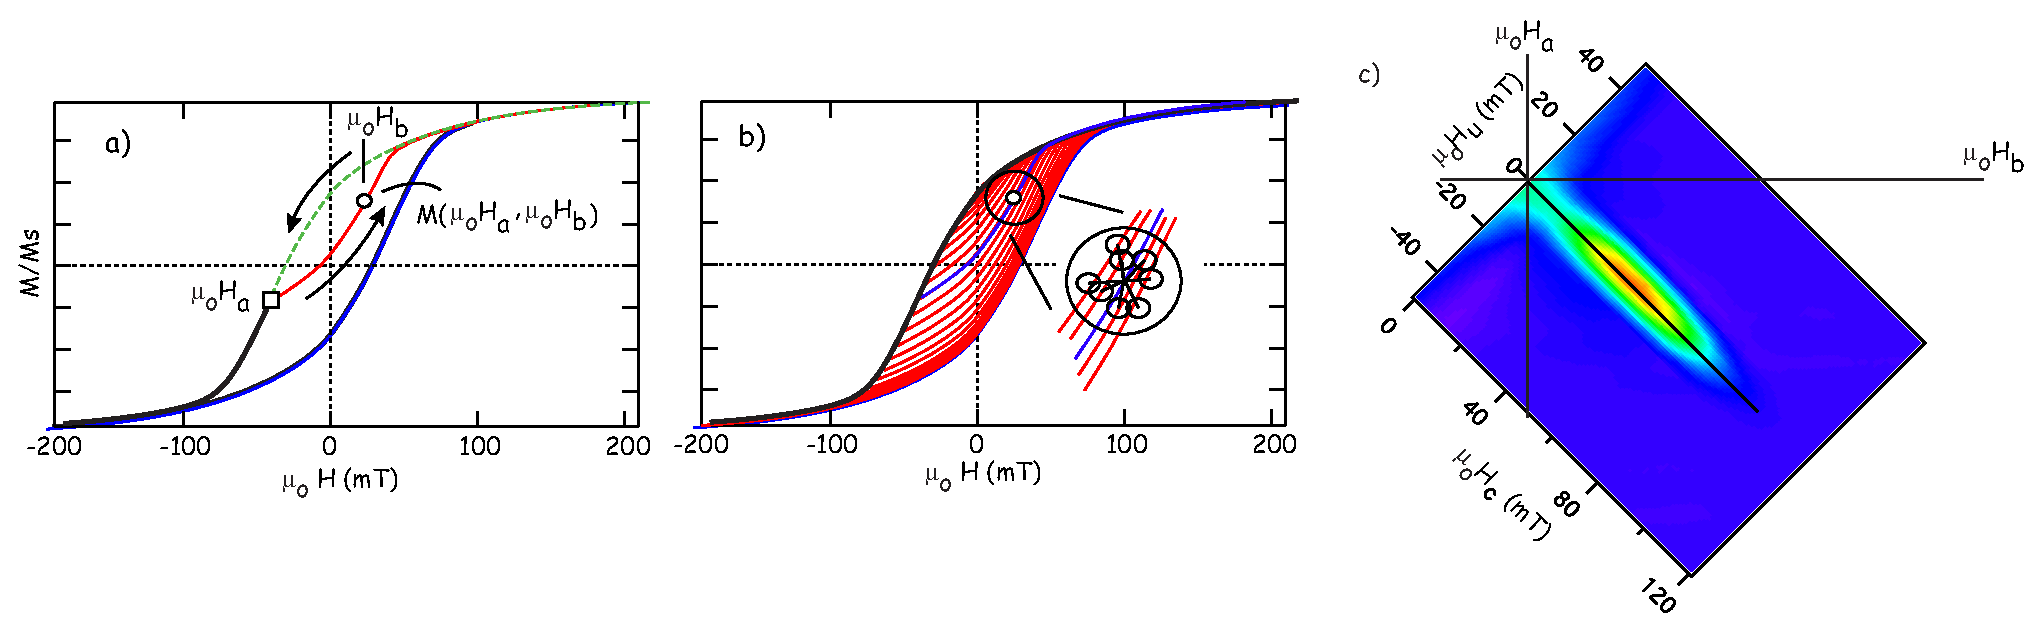
\includegraphics[width=14 cm]{EPSfiles/forcprinc.eps}
\caption{a) Dashed line is the descending magnetization curve taken from a saturating field to some field $H_a$.  Red line is the first order reversal curve (FORC) from $H_a$ returning to saturation.   At any field $H_b>H_a$ there is a value for the magnetization $M(H_a,H_b)$.  b) A series of FORCs for a single domain assemblage of particles.  At any point  there are a set of related ``nearest neighbor'' measurements (circles in inset).  A least-squares fit to Equation 5.8 can be determined for each point.    c) A contour plot of the FORC density surface for data in b).   Specimen is  of the Tiva Canyon Tuff, courtesy of the Institute for Rock Magnetism.   }
\label{fig:forcprinc}
\end{figure}


Hysteresis ratios of mixtures of SD and MD particles will also plot in the ``PSD'' box.  Dunlop (2002a) derived the theoretical behavior of such mixtures on the Day diagram.    The key equations are 1) Equation 9 from Dunlop (2002) which governs the behavior of the ratio $M_r/M_s$ as a function of the volume fraction of single domain material ($f_{SD}$) and multi-domain material ($f_{MD}$): 

$$
{M_r/M_s} = f_{SD} (M_r/Ms)_{SD} + f_{MD} (M_r/M_s)_{MD}, 
$$

\noindent   2) Equation 10 from Dunlop (2002a) which governs the behavior of coercivity:

$$
H_c = [f_{SD} \chi_{SD} (H_c)_{SD} + f_{MD} \chi_{SD} \chi_{MD} (H_c)_{MD}] / (f_{SD} \chi_{SD} + f_{MD} \chi_{MD}), 
$$

\noindent and 3) Equation 11 from Dunlop (2002a) which governs the behavior of coercivity of remanence in SD/MD mixtures:

$$
{H_{cr} =}  {  f_{SD}( \chi_r)_{SD} (H_{cr})_{SD} +  f_{MD}( \chi_r)_{MD} (H_{cr})_{MD} } \over { f_{SD} (\chi_r)_{SD} + f_{MD} (\chi_r)_{MD} }
$$

\noindent where $\chi_{SD}$ and $\chi_{MD}$ are the susceptibilities of the SD and MD fractions respectively and $(\chi_r)_{SD}$  and $(\chi_r)_{MD}$ are the $M_r$ vs $H_{cr}$ slopes of the SD and MD remanences respectively.   What we need to calculate the SD/MD mixing curve are values for the  various parameters  for single domain and multi domain end-members.   These were measured empirically for the MV1H bacterial magnetosomes (see Chapter 6) and  commercial magnetite (041183 of Wright Company) by    Dunlop and Carter-Stiglitz (2006) \nocite{dunlop06}  and shown in Table~\ref{tab:end members}.    Using the linear mixing model of Dunlop (2002a), we  plot the theoretical mixing curve predicted for these empirically constrained  end-members as the heavy red line in Figure~\ref{fig:md}c.    

\begin{table}
\caption{Empirical values for hysteresis parameters measured for single domain (SD) and multi-domain (MD) end-members of  Dunlop and Carter-Stiglitz (2006).}
\label{tab:endmembers}
\begin{tabular}{ llllll   }
\hline
SD/MD& $M_r/M_s$ & $\chi$ (A m$^{-1}$T$^{-1}$) & $\chi_r$ (MA m$^{-1}$T$^{-1}$)&$ \mu_o H_c$ (mT) &$ \mu_o H_{cr}$ (mT)\\
\hline
SD & 0.5 &  5.2&  4.55&46 & 52.5\\
MD & 0.02 & 4.14 & 0.88 &5.56 &26.1\\
\hline
\end{tabular}
\end{table}



% but the relationships are highly non-linear and are solved by trial and error.    Moreover, there are many embedded (and untestable) assumptions involved in these curves.      

If a population of SD particles are so closely packed as to influence one another, there will be an effect of particle interaction.  This will also tend to suppress the $M_r/M_s$ ratio, drawing the hysteresis ratios down into the PSD box.  
Finally, the PSD box could be populated by pseudo-single domain grains themselves.  Here we will dwell for a moment on  the meaning of the term ``pseudo-single domain'', which  has evolved from the original posed by 
\index{Stacey, F.}
Stacey (1961; see  discussion in 
\nocite{tauxe02}
\index{Tauxe, L.}
Tauxe et al. 2002). \nocite{stacey61,tauxe02}  In an attempt to explain trends in TRM acquisition Stacey envisioned that irregular shapes caused unequal domain sizes, which would give rise to a net moment that was less than the single domain value, but considerably higher than the very low efficiency expected for large MD grains.    The modern interpretation of PSD behavior is complicated micromagnetic structures that form between classic SD (uniformly magnetized grains) and MD (domain walls) such as the flower or vortex remanent states (see, e.g., Figure~\ref{fig:nonuniform} in Chapter 4).   
Taking all these factors into account means that interpretation of the Day diagram is far from unique.   The simple calculations of Dunlop (2002a) are likely to be  inappropriate for almost all natural samples.  






\section{First order reversal curves}


Hysteresis loops can yield a tremendous amount of  information yet much of this is lost by simply estimating the set of parameters $M_r, M_s,  H_{cr}, H_c, \chi_i, \chi_{hf}$, etc.   
\nocite{mayergoyz86}
\index{Mayergoyz, I.D.}
Mayergoyz (1986)    developed a method using  what are known as   {\it First Order Reversal Curves} or FORCs to represent hysteresis data.  The most recent way of dealing with
\index{diagrams!FORC}
 FORCs is that of
 \nocite{harrison08}
 \index{Harrison, R.J.}
 \index{Feinberg, J.M.}
  Harrison and Feinberg (2008)  which is illustrated in Figure~\ref{fig:forcprinc}.  In the FORC experiment,  a specimen is subjected to a saturating field,  as in most hysteresis experiments.  The field is lowered to some field $\mu_oH_a$, then increased again through some value $\mu_oH_b$  to saturation (see Figure~\ref{fig:forcprinc}a).   The magnetization curve between $\mu_o H_a$ and $\mu_oH_b$ is a ``FORC''.  A series of FORCs (see Figure~\ref{fig:forcprinc}b) can be generated to the desired resolution.  


 
 \begin{figure}[h!b]
%\epsfxsize 14cm
%\centering \epsffile{EPSfiles/m428.eps}
\centering  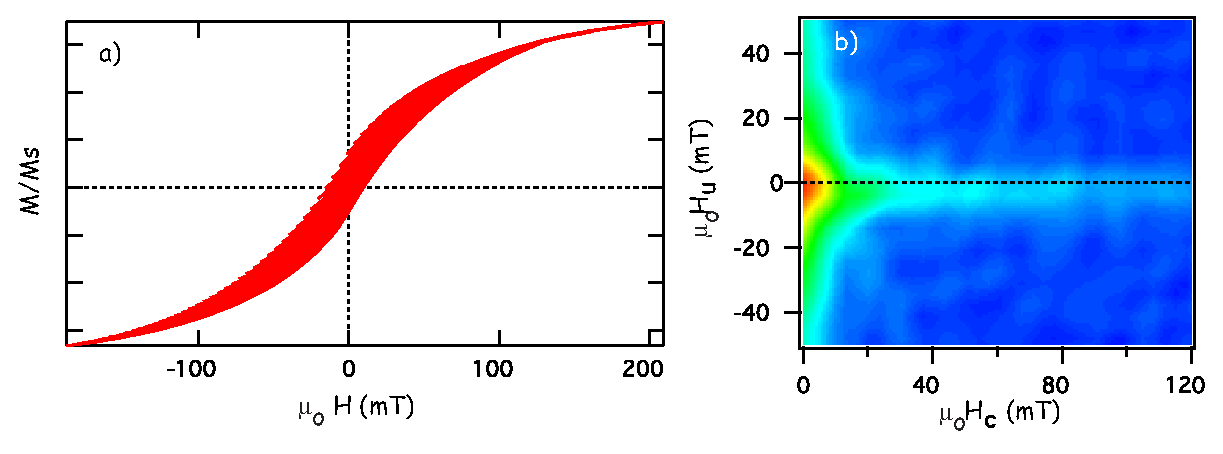
\includegraphics[width=14 cm]{EPSfiles/m428.eps}
\caption{a)  A series of FORCs for a ``pseudo-single domain'' specimen.  b) FORC diagram for data in a).   Specimen  is  of the Stillwater Layered Intrusion, courtesy of J.S. Gee.   }
\label{fig:forcpsd}
\end{figure}


To transform FORC data into some useful form, Harrison and Feinberg (2008) use a locally-weighted regression smoothing technique (LOESS).   For a given measurement point $P$ LOESS fits a second-order polynomial function of the form

\begin{equation}
M(H_a,H_b)= a_1 + a_2H_a + a_3H_a^2 + a_4H_b +a_5H_b^2 +a_6H_aH_b,
\label{eq:forc}
\end{equation}

\noindent  to the measured magnetization surface in a specified region (for example the circle shown in Figure~\ref{fig:forcprinc}b) where the $a_i$ are fitted coefficients.     The LOESS technique takes a user defined number of  the nearest neighbors (see inset to Figure~\ref{fig:forcprinc}b) for an arbitrary shaped region over which the data are smoothed.    
The coefficient $-a_6(H_a,H_b)$ is  the FORC density at the point.    A FORC diagram is the contour plot  of the FORC densities, rotated such that $\mu_oH_c = \mu_o(H_b-H_a)/2$ and $\mu_oH_u = \mu_o(H_a+H_b)/2$.    Please note that because $H_a<H_b$, data are only possible for positive $H_c$.  
 

\begin{figure}[htb]
%\epsfxsize 10cm
%\centering \epsffile{EPSfiles/ZFORC.eps}
\centering  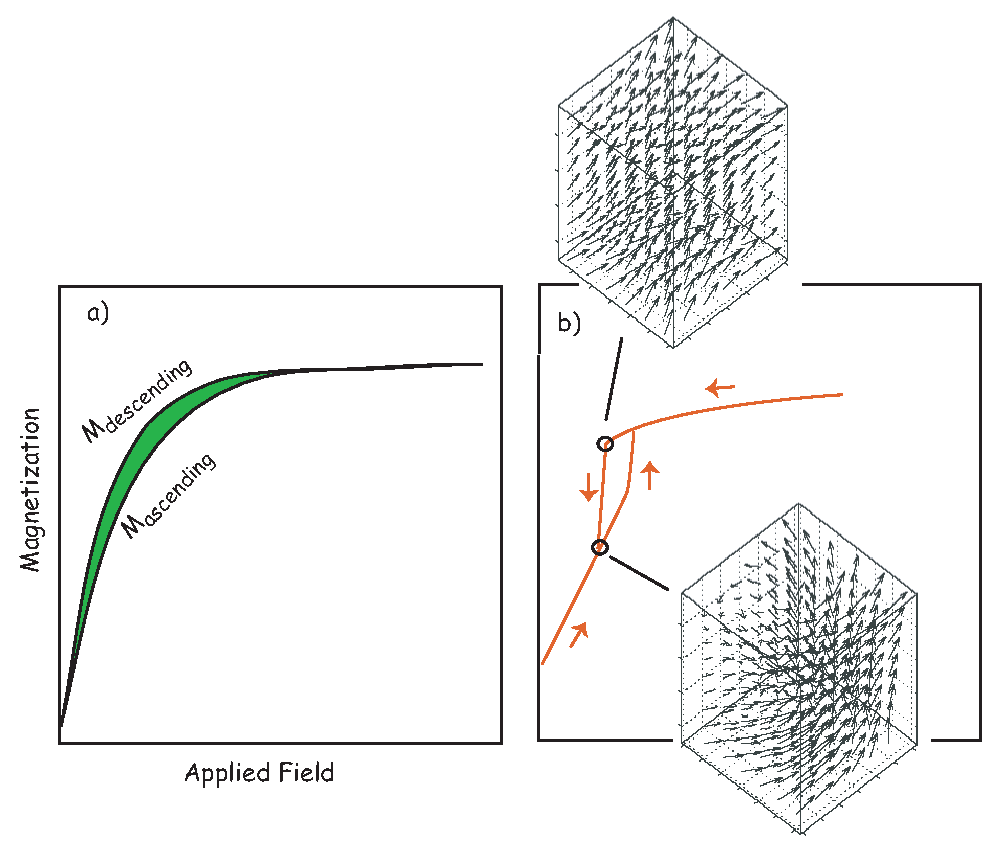
\includegraphics[width=10 cm]{EPSfiles/ZFORC.eps}
\caption{a) Illustration of a Zero FORC (ZFORC) whereby the descending loop from saturation is terminated at zero field and the field is then ramped back up to saturation.  The  transient hysteresis (TH) of 
Fabian (2003) is the shaded area between the two curves.  b) Micromagnetic model of a ZFORC for a 100 nm cube of magnetite.  Two snap shots of the internal magnetization on the descending and ascending loops are shown in the insets.  [Figure redrawn from Yu and Tauxe, 2005.] }
\label{fig:ZFORC}
\end{figure}
\nocite{yu05b}
\nocite{fabian03} 

 Imagine we travel down the descending magnetization curve (dashed line in Figure~\ref{fig:forcprinc}a) to a particular field $\mu_o H_a $ less than the smallest flipping field in the assemblage.   If the particles are single domain, the behavior is reversible and the first  FORC will travel back up the descending curve.  It is only when $|\mu_o H_a|$ exceeds the flipping field of some of the particles that the FORC will trace a new curve on the inside of the hysteresis loop.  In the simple single domain, non-interacting,  uniaxial magnetite case, the FORC density in the quadrants where $H_a$ and $H_b$ are of the same sign must be zero. Indeed, FORC densities will only be non-zero for the range of flipping fields  because these are the bounds of the flipping field distribution.      So the diagram in Figure~\ref{fig:forcprinc}c is nearly that of an ideal uniaxial SD distribution.  
 
 Consider  now the case in which a specimen has magnetic grains with non-uniform magnetizations such as vortex structures or domain walls.   Walls and vortices can move much more easily than flipping the moment of an entire grain coherently.  In fact,  they begin to move in small jumps (from LEM to LEM) as soon as the applied field changes.  If a structure nucleates while the field is decreasing and  the field is then ramped back up, the magnetization curve will not be reversible, even though the field never changed sign or approached the flipping field for coherent rotation.   The resulting FORC for such behavior would have much of the ``action'' in the region where $H_a$ is  positive.   When transformed to $H_u$ and $H_c$, the diagram will have the high densities for small $H_c$ but over a range of  $\pm H_u$.  The example shown in   Figure~\ref{fig:forcpsd} is of a specimen that has been characterized as ``pseudo-single domain''.  The FORC diagram in Figure~\ref{fig:forcpsd}b has some of the FORC densities concentrated along the $H_c$ axis characteristic  of single domain specimens (e.g., Figure~\ref{fig:forcprinc}c), but there is also concentration along the $H_u$ axis characteristic of PSD and MD specimens.       
 



  In many cases the the most interesting thing one learns from FORC diagrams is the degree to which there is irreversible behavior  when the field is reduced to zero then ramped back up to saturation (see Figure~\ref{fig:ZFORC}).  Such irreversible behavior in what 
  \nocite{yu05b} 
  \index{Yu, Y.}
  \index{Tauxe, L.}
  Yu and Tauxe (2005) call the ``Zero FORC'' or ZFORC  can arise from particle interactions, domain wall jumps or from the formation and destruction of vortex structures in the magnetic grains.   

\nocite{fabian03} 
\index{Fabian, K.L.}
Fabian (2003) defined a parameter called ``transient hysteresis''  which is the area between the ascending and descending loops of a ZFORC (shaded area in Figure~\ref{fig:ZFORC}).    This is defined as:

$$
TH= \mu_o\sum_0^{H_s} [M_{descending} - M_{ascending}] \cdot \Delta H.
$$
\noindent  where $\Delta H$ is the field increment used in the hysteresis measurement.   When normalized by $M_s$, TH has units of tesla.    
Transient hysteresis is thought to result  from self demagnetization, for example  shifting of domain walls or the formation and destruction of vortex structures.  An example of what might be causing transient hysteresis at the macro scale is shown for micromagnetic modelling of a  single particle in Figure~\ref{fig:ZFORC}b 
\nocite{yu05b}
\index{Yu, Y.}
\index{Tauxe, L.}
(Yu and Tauxe, 2005).   The ZFORC starts and ends at saturation.  On the descending loop, a vortex structure suddenly forms, at the point on the hysteresis loop labelled a), sharply reducing the magnetization.  The magnetization state just before the jump is shown as snapshot labelled ``descending branch''.  The vortex remains along the  ascending branch until much higher fields (see snapshot labelled ``ascending branch'').  The irreversible behavior of millions of particles with different sizes and shapes leads to the total transient hysteresis of the macro specimen.    
In general,  Yu and Tauxe  (2005) showed that the larger the particle, the greater the transient hysteresis, until truly multi-domain behavior essentially closed the loop, precluding the observation of TH (or of a FORC diagram for that matter). 

\vskip .5 in\noindent{SUPPLEMENTAL READING:} Dunlop and \"Ozdemir (1997), chapters 5 and 11;  O'Reilly (1984), pp 69-87;  \nocite{oreilly84}
 Dunlop (2002a,b) \nocite{dunlop02b,dunlop02a}

\vskip 24pt

\section{Problems}

In this set of problems, we will begin to use REAL data.  The data files used with this book are part of the {\bf PmagPy} distribution, which you should have already downloaded and installed.  Look in the Datafile directory under `Essentals\_Examples' and you will find what you need.  
%LJ  replaced .http://magician.ucsd.edu/~ltauxe/RockNPmag/Datafiles.zip with above for less confusion

{\parindent 0pt \parskip 12pt 


{\bf Problem 1}

For a grain with uniaxial anisotropy in an external field, the direction of magnetization in this grain will be controlled entirely by the uniaxial anisotropy energy density  $\epsilon_a$ and the magnetic interaction energy $\epsilon_m$.  The total energy can be written:

$$
\epsilon_{tot} = \epsilon_a + \epsilon_m = K_u \sin^2 \theta - \mu_o H M_s \cos (\phi -\theta),
$$
\noindent where $\phi$ is the angle of the applied field relative to the easy axis of magnetization and $\theta$ is the angle of the moment relative to the easy direction.  Show that the flipping field of  a grain whose moment is initially antiparallel to the field, i.e. $\phi$ = 180$^{\circ}$,  is given by:
$$
{H_c =} { {2K_u}\over {\mu_o M_s}}.
$$


\begin{figure}[htb]
%\epsfxsize 13.5cm
%\centering \epsffile{EPSfiles/gui-3.eps}
\centering  \includegraphics[width=13.5 cm]{EPSfiles/gui-3.eps}
\caption{Various hysteresis plots.}   
\label{fig:gui}
\end{figure}


{\bf Problem 2}

In this problem, you will become familiar with the {\bf  QuickMagIC.py} graphical user interface (GUI) for some of the {\bf PmagPy}  programs most useful to the working paleomagnetist.   These programs are designed to work with the Magnetics Information Consortium (MagIC)  database (see \url{http://earthref.org/MAGIC}; see also  \href{http://earthref.org/PmagPy/cookbook}{PmagPy} documentation) -- a database designed for paleomagnetic and rock magnetic measurements.  For now we are just using a few of the  programs.   

  Someone has measured  hysteresis loops  on a mysterious set of specimens using an alternating gradient force magnetometer.     These are contained in the Chapter\_5 directory of the Datafiles package you downloaded.  

{\bf QuickMagIC.py} wants its own directory to store and manipulate files, so create a new directory (inside the Chapter\_5 directory for convenience).  From the command line, type {QuickMagIC.py}.    Choose your new directory by clicking on the `change dir' button.     DO NOT use directories with spaces in the path name (this is common on PCs).    


On the menu bar of the {\bf QuickMagIC.py} GUI you will find a pull down menu labelled ``Import''.  Select ``Hysteresis Files'' and choose the `Import entire directory'' option.  Choose the Chapter\_5 datafile directory.    When prompted, select the cgs units option.  These data are hysteresis loops that were measured with the ``old'' file format, so do not select ``new format''.   If you were really uploading a data  into the database, you would  fill out the location and other helpful information but for now, just click on the ``OK'' button to accept the specimen name.  {\bf QuickMagIC.py} copies  each datafile to the project directory and converts it to the MagIC format.  Repeat the file importation procedure for all the files in the Chapter\_5 directory.    When you have finished importing the files, click on the  ``convert magnetometer files...'' on the main panel and select the `Next step' button.  This finds all the individual measurement files and clicking 'OK' will combine them into a single file called {\it magic\_measurements.txt}.   




a) On your command line, change directories into the Project Directory you just created and type `hysteresis\_magic.py -f magic\_measurements.txt'.  This will  read in your datafile specimen by specimen, making plots and collecting hysteresis parameters.   To advance through the plots, just press return after each plot until finished.   Your terminal may look something like Figure~\ref{fig:gui}.    
Write a detailed figure caption for the three non-blank figures for specimen IS06a-2.   What is the difference between the red and blue lines?   What are the blue squares?  What is the ``DeltaM'' curve. 

b)  Stepping through all the plots in the last problem created a file that stored the hysteresis parameters like saturation remanence, coercivity, etc. in a file called \newline  {\it  rmag\_hysteresis.txt} in the project directory.    Now type `dayplot\_magic.py'     Write a caption for these plots.  How would you interpret them?  


}
